\section{Módulo de conexión}

El módulo de conexión se encarga de lanzar los módulos de análisis y/o el de composición, según la demanda del usuario. Para ello, debe ejecutar los correspondientes programas asociados a cada módulo, de tal forma que la vista de despliegue es tal y como muestra la Figura~\ref{fig:muphic-deploy-diagram}.\\


		\begin{figure}[!htbp]
		\centering
		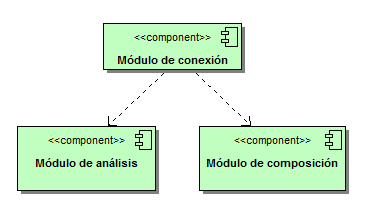
\includegraphics[scale=0.6]{graphics/muphic-deploy-diagram.png}
		\caption{Diagrama de despliegue del módulo de interconexión}
		\label{fig:muphic-deploy-diagram}
		\end{figure}
		
Es aquí donde surge el principal problema de que la aplicación sea multiplataforma, ya que distintos sistemas operativos, como Windows o los basados en UNIX, proponen distintas maneras de lanzar archivos ejecutables. Para solventar estos problemas, se han concentrado las consiguientes diferencias del código para cada sistema operativo en la clase \emph{Launcher}, como se ve en la Figura~\ref{fig:muphic-class-diagram}.\\

		\begin{figure}[!htbp]
		\centering
		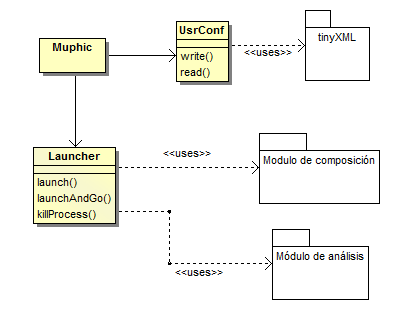
\includegraphics[scale=0.6]{graphics/muphic-class-diagram.png}
		\caption{Diagrama de clases del módulo de interconexión}
		\label{fig:muphic-class-diagram}
		\end{figure}
		
La clase Launcher ofrece funcionalidad para ejecutar una aplicación interrumpiendo la ejecución en curso (\emph{Launcher::launch()}), o bien en paralelo (\emph{Launcher::launchAndGo()}), así como para detener la ejecución de un programa lanzado (\emph{Launcher::killProcess()}). De esta forma, la totalidad del resto del código del proyecto se ha realizado sin preocuparse de la plataforma de ejecución, delegando de Launcher siempre que era necesario realizar operaciones propias de cada sistema operativo.\\

En la Figura~\ref{fig:muphic-sec-diagram} se muestra un ejemplo de ejecución del módulo, en el que se ejecutan tanto el módulo de análisis como el de composición.\\

		\begin{figure}[!htbp]
		\centering
		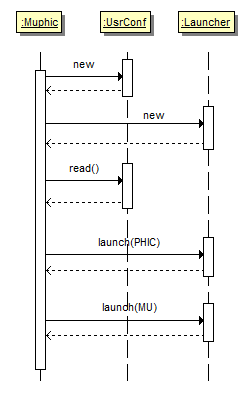
\includegraphics[scale=0.6]{graphics/muphic-sec-diagram.png}
		\caption{Diagrama de flujo del módulo de interconexión}
		\label{fig:muphic-sec-diagram}
		\end{figure}
		
Cabe destacar en esta sección el uso de la clase \emph{UsrConf}, encargada de administrar el archivo de configuración del completo proceso de análisis y composición. Este archivo, estructurado en forma de XML, contiene tanto los parámetros necesarios para la ejecución del módulo de análisis (vistos en la Sección~\ref{sec:algAnalisis}) como los necesarios para la ejecución del módulo de composición. Además, permite indicar qué módulo se debe ejecutar, de forma que se puede ejecutar únicamente uno de los dos módulos o los dos a la vez. La clase \emph{UsrConf} ofrece funcionalidad para escribir y leer (ya sea en su totalidad o la parte relativa a un único módulo) el archivo XML.

\section{Interfaz Gráfica}

\todo{rehacer reusando parte de esto:

El desarrollo de la interfaz gráfica se decidió realizar a través de un framework que facilitase la construcción de la misma. Qt, la herramienta que se utilizó se eligió debido a dos criterios, era multiplataforma, al igual que la aplicación, servía para trabajar con móviles, siguiendo así uno de los enfoques iniciales del proyecto que más adelante fue descartado. Además Qt trabaja con C++ como lenguaje de programación, el mismo que el núcleo de la aplicación y ofrece facilidades a la hora de integrar audio, a través de la librería Phonon, o componentes personalizados en una interfaz.\\
\todo{Este párrafo no se si abriría mejor la parte de arquitectura}
\newline
La interfaz esta compuesta de tres pestañas cada una encargada de una parte de la funcionalidad:

\underline{Composition Config:}
\\En esta pestaña se pueden encontrar todas las opciones disponibles para el compositor musical, estás serán transmitidas a los módulos de la aplicación cuando se pulse el botón de "Compose" en la "Main Window" a través del documento XML mencionado anteriormente.
\\Como se puede ver en la imagen adjunta, hay opciones para cuatro voces, que son aquellas con las que trabajan los compositores de la aplicación siendo, normalmente, la "Voice 1" la melodía principal, la "Voice 2" un acompañamiento, la "Voice 3" el bajo y la "Voice 4" la percusión. Las opciones disponibles son las siguientes:
\\\todo{Adjuntar imagen}
\newline
\\textit{Color System:} Hace referencia referencia a la teoría sinestésica que se utilizará como base para la relación de color-notas durante la composición musical.
\\textit{Composer:} En las cuatro voces se refiere a que compositor se utilizará para esa voz, al presionarlo se desplegarán los distintos compositores que están disponibles para que el usuario elija el que mejor le convenga.
\\textit{Instrument:} En las cuatro voces se refiere a que instrumento se utilizará para esa voz en concreto, al presionarlo se desplegarán los instrumentos disponibles.
\\textit {Composer Mixer:} Hace referencia a que como se combinarán las cuatro voces anteriores.
\\textit{Tempo:} 
\\\todo{A rellenar con gente que sepa describirlo mejor que yo. \\También hay que repasar lo anterior}
\newline
\\{\bf Libreria Phonon}
\\Esta es una librería proporcionada por Qt para la reproducción de audio, al ser un módulo externo requiere una serie de librerías añadidas que están incluidas en el paquete de instalación de windows, sin embargo tendrán que ser instaladas en linux utilizando alguno de los gestores de software disponibles realizando una búsqueda con la palabra clave: Phonon.
\\Las librerías requeridas son las siguientes: (LISTA DE LIBRERÍAS)
\\En el caso de que no funcione el sistema de reproducción, se pueden encontrar los archivos de audio en la ruta especificada en "Midi Output"
\newline
\\\todo{Claramente esta parte va en arquitectura, sin embargo no se que más comentar de la arquitectura de la GUI puesto que casi todo esta hecho con QT, como no digamos el widget de carlos...}
\\La interacción con phonon se realiza utilizando la funcionalidad proporcionada por el framework. Se asocia el fichero multimedia a un tipo proporcionado por Phonon que a su vez lo conecta con el sistema de audio predeterminado para cada sistema operativo.
\\El uso de Phonon es conveniente porque a pesar de sus complicaciones ofrece una manera sencilla de incluir un reproductor en la interfaz, que a su vez, es multiplataforma sin obligar al usuario a buscar el archivo de audio o forzar una llamada a un tercer programa que reproducir la música que generada.

\subsection{Uso de la librería Qt}

\todo{Hacer, usar parte de 3.3.6}

\subsection{Vista general}

\todo{Hacer, usar parte de 3.3.6}

\subsection{Widget Gráfico}

\todo{Hacer}

\subsection{Uso de la librería Phonon}

\todo{Hacer, usar parte de 3.3.6}

La interfaz para poder reproducir los archivos de audio generados hace uso de una librería externa proporcionada por Qt, se trata de Phonon \cite{phononOverview}. }